\documentclass[10pt]{article}
\usepackage{amssymb}
\usepackage{amsthm}
\usepackage[fleqn]{amsmath}
\usepackage{listings}
\usepackage{color}
\usepackage{graphicx}
\usepackage{subcaption}

\lstdefinestyle{matlab-style}{
language=Matlab,
basicstyle=\scriptsize\ttfamily,
tabsize=2,
rulecolor=,
language=matlab,
basicstyle=\scriptsize,
aboveskip={1.5\baselineskip},
columns=fullflexible,
showstringspaces=false,
extendedchars=true,
breaklines=true,
prebreak = \raisebox{0ex}[0ex][0ex]{\ensuremath{\hookleftarrow}},
frame=single,
showtabs=false,
showspaces=false,
showstringspaces=false,
identifierstyle=\ttfamily,
keywordstyle=\color[rgb]{0,0,1},
commentstyle=\color[rgb]{0.133,0.545,0.133},
stringstyle=\color[rgb]{0.627,0.126,0.941},
keepspaces=true,
numbers=left,
numbersep=5pt,
numberstyle=\tiny\color[rgb]{0.5,0.5,0.5},
stepnumber=1
}

\newcommand{\bs}[1] {\boldsymbol{#1}}

\title{Optimizing a wing spar under uncertaintity \\MANE 6963 - Project 3}
\author{ID: 2168}
\date{}

\begin{document}

\maketitle

\section{Executive summary}

In this report we investigate the optimal design of a
wing spar as the primary support for the wing of an
aircraft when loading conditions to the wing are uncertain.
Our main objective is to reduce the weight of the spar
by at least $70$ percent when compared to a nominal design,
while still maintaining a safe
design for various loading conditions on the wing.
This goal was achieved using optimization under design
uncertainty by ensuring that the stress distribution
over the optimal spar geometry remains within an
acceptable safety range. To perform the optimization
under uncertainty, the following Matlab routines
were implemented: 
\emph{CalcWeight.m}, \emph{CalcQPs.m},
\emph{StressConstraints.m}, \emph{Plotter.m}
\emph{Driver.m},
and are listed in the Appendix.
Figure \ref{fig:spar} provides an illustration of the
spar that is to be designed.

\begin{figure}[hbt]
\centering
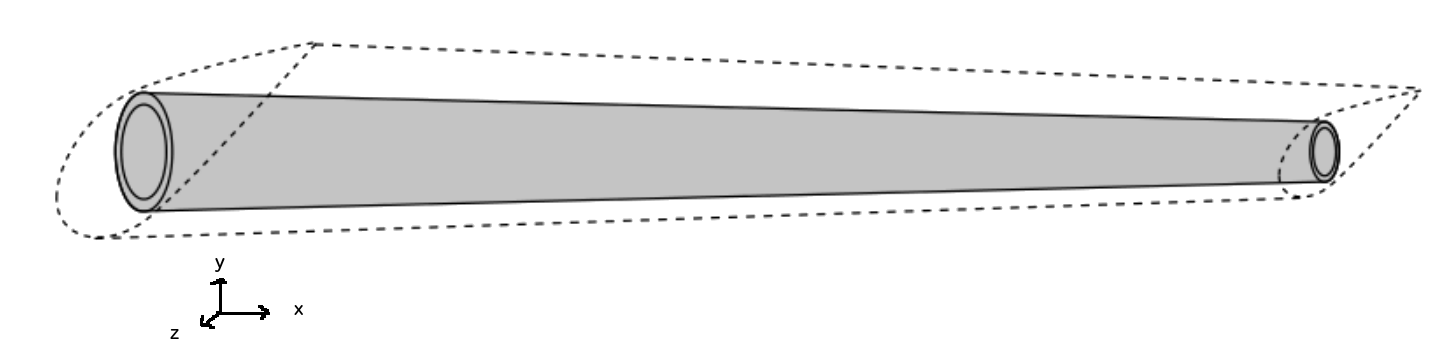
\includegraphics[width=0.6\textwidth]{spar}
\caption{Wing (dotted lines) and illustration of spar geometry}
\label{fig:spar}
\end{figure}

This report is structured as follows: First
we present an overview of the operational assumptions
of the aircraft and constraints imposed on wing spar.
Next, we present an overview of the geometry parameterization.
Then we outline the basic analysis methods used to compute
stress distributions along the spar. We provide
an overview of the optimization problem statement, the
methods used to solve the optimization problem, and
details on the software implementation for optimization routines.
Finally, we discuss results obtained by solving the
optimization problem.

\section{Assumptions and design constraints}

\subsection{Aircraft operational assumptions}

We assume that the total mass of the aircraft is
$m_{\text{plane}} = 500$ kg and that the weight of the
plane is equally supported by two wings. The length
of the spar is denoted by $L$, and the weight of the
plane is given as
$w = (9.81 \text{m} \, \text{s}^{-1}) (500 \text{kg})$.
Additionally, we assume that the plane is operating
during a maneuver during which there is uncertainty in
the loading on the wing. This uncertain loading can be
described as a function of the random parameters $\xi_n$,
where $n=1,2, \dots, 4$, as:
%
\begin{equation}
F(x, \bs{\xi}) = F_{\text{nom}}(x) + \delta_F(x, \bs{\xi}).
\label{eq:pert_force}
\end{equation}
%
Here $F_{\text{nom}}(x)$ is a baseline linearly
distributed loading given by:
%
\begin{equation}
F_{\text{nom}}(x) = \frac{2.5 w}{L}(1 - \frac{x}{L}),
\end{equation}
%
and $\delta_F(x, \bs{\xi})$ is an uncertain perturbation to
the loading, given as
%
\begin{equation}
\delta_F(x, \bs{\xi}) = \sum_{n=1}^{4} \xi_n
\cos \left( \frac{(2n-1) \pi x}{2L} \right).
\end{equation}
%
Each random variable $\xi_n$ is assumed to be
normally distributed with mean $0$ and standard deviation
$\frac{F_\text{nom}(0)}{10n}$, for $n=1,2,\dots,4$, such
that
%
\begin{equation}
\xi_n \sim
\mathcal{N} \left( 0, \frac{F_\text{nom}(0)}{10n} \right).
\end{equation}
%

\subsection{Engineering design assumptions}

We assume that the wing semi-span $L$ is $7.5$ m, and that
the spar supporting the wing will be made out of a carbon
fiber composite material. The material properties of the
composite are listed in Figure \ref{fig:materials}.
Additionally, we assume that the cross-section of the
spar in the $yz$ plane is a circular annulus.

\begin{figure}[hbt]
\centering
\begin{tabular}{ | l | r  |}
\hline
Material property & Value \\ \hline
Density $(\rho)$ & $1600$ km/m$^3$ \\ \hline
Young's modulus $(E)$ & $70$ GPa \\ \hline
Ultimate yield strength $(Y)$ & $600$ MPa \\ \hline
\end{tabular}
\caption{Material properties of the spar}
\label{fig:materials}
\end{figure}

\subsection{Engineering design constraints}

Due to the material manufacturing constraints, we assume
that the inner radius of the spar $r^i$ at all points
along the $x$-axis is greater than or equal to $1$ cm
and that the inner and outer radii of the spar cannot
be more than $2.5$ mm apart. Because the spar must
remain within the wing, we constrain the outer radius
$r^o$ of the spar to be less than or equal to $5$ cm.
Finally, we stipulate that the expected value
$\text{E}[s(x, \bs{\xi})]$  of
the normal stress $s$ at all span-wise locations
plus six standard
deviations of the stress must remain below the yield
strength in order to maintain a safe design. That is,
%
\begin{equation}
\text{E} [ s(x, \bs{\xi}) ] + 6 \sqrt{\text{Var}[s(x, \bs{\xi})]}
\leq Y,
\end{equation}
%
Here the expected value of the stress is given by
%
\begin{equation}
\text{E}[ s(x, \bs{\xi}) ] =
\iiiint _{X} s(x, \bs{\xi}) \prod_{n=1}^{4} P(\xi_n, \mu_n, \sigma_n)
\, \text{d} \xi_1
\, \text{d} \xi_2
\, \text{d} \xi_3
\, \text{d} \xi_4,
\label{eq:expected}
\end{equation}
%
where $X = [-\infty,\infty]^4$ and $P(\cdot,\cdot,\cdot)$ denotes
the random variables' probability density function.
As mentioned previously, the mean $\mu_n$ for each random variable
is $0$ and
the standard deviation $\sigma_n$ for each random variable
is given as $\sigma_n = \frac{F_{\text{nom}}(0)}{10n}$.
The variance of the stress is given as
%
\begin{equation}
\text{Var}[s] = \text{E}[s^2] - \text{E}[s]^2.
\end{equation}

\section{Geometry parameterization}

As previously stated, each cross-section in the $yz$
plane of the spar geometry is assumed to be a circular
annulus. We discretize the $x$-axis using $N_x$
grid points and assume the spar varies piecewise
linearly along the $x$-direction from grid point
to grid point. The vector $\bs{p} \in \mathbb{R}^{2 N_x}$
is used to denote the design parameter variables that
is a concatenated vector of inner radii $r^i_j$
and annular thickness values $t_j = r^o_j - r^i_j$,
evaluated at the discrete grid points $x_j$,
where $j=1,2,\dots,N_x$. The vector $\bs{p}$ has the
layout
%
\begin{equation}
\bs{p} = [r^i_1, r^i_2, \dots r^i_{N_x}, t_1, t_2, \dots, t_{N_x}]^T.
\end{equation}

\section{Analysis methods}

The deformation of the wing spar is modeled using Euler-Bernoulli
beam theory, represented by the PDE:
\begin{equation}
\frac{d^2}{d x^2}
\left( E I_{yy} \frac{d^2 u}{dx^2} \right) =
F(x, \bs{\xi}), \quad \forall x \in [0,L],
\label{eq:pde}
\end{equation}
with zero displacement boundary and zero angular
displacement boundary conditions imposed at
$x=0$ and traction free boundary conditions
imposed at $x=L$. Here $I_{yy} = \frac{\pi}{4}( (r^o)^4 - (r^i)^4)$
represents the second moment of inertia.
The perturbed applied loading force $F(x, \bs{\xi})$
is computed by the Matlab routine
\emph{CalcPertForce.m} to agree with equation
\eqref{eq:pert_force}.
The model PDE is solved via finite element analysis, with
$N_x-1$ elements. The stresses at grid points $s_j$ are then
found via a post-processing step that uses the computed displacements
$u_j$.
The correctness of the finite element analysis
has been verified by a previous project. We do not repeat the
verification and validation of the analysis here for the sake
of brevity.

\section{Optimization methods}

\subsection{Optimization problem}

Let $m(\bs{p})$ denote the mass of the spar with an explicit
dependence on the design parameters $\bs{p}$. The optimization
problem we are interested in solving can then be stated as:
%
\begin{equation*}
\begin{aligned}
& \underset{\bs{p}}{\text{minimize}}
& & m(\bs{p}) \\
& \text{subject to}
& & p_j \geq 0.01,                    &j=1,2,\dots,N_x \\
&&& p_{N_x+j} \geq 0.0025,            &j=1,2,\dots,N_x\\
&&& p_j + p_{N_x +j} \leq 0.05,       &j=1,2,\dots,N_x \\
&&& \left(\text{E}[s_j(\bs{p})] + 6 \sqrt{\text{Var}[s_j(\bs{p})] } \right) / Y \leq 1.0, 
 &j=1,2,\dots,N_x
\end{aligned}
\label{eq:optim}
\end{equation*}

The entirety of the optimization problem is
contained in the Matlab script \emph{Driver.m}. This script utilizes
Matlab's \emph{fmincon} routine to perform gradient-based optimization.
We choose \emph{fmincon}'s `SQP' (sequential quadratic programming)
algorithm with default convergence tolerances. Additionally,
we provide \emph{fmincon} the  objective gradient $\nabla m (\bs{p})$
and the gradient of the nonlinear stress constraints as computed
by the complex step method.

\subsection{Implementation details}

The objective mass of the spar is computed by the Matlab routine
\emph{CalcWeight.m} as:
%
\begin{equation}
m(\bs{p}) = \pi \rho \int_0^L \left[ (r^0)^2 - (r^i)^2 \right] \text{d} x.
\end{equation}
%
The method \emph{CalcWeight.m} returns both the value of the
mass $m$ and its gradient $\nabla m$ as computed by the complex
step method
%
\begin{equation}
[ \nabla m(\bs{p}) ]_j = \frac{\text{Im}(m( \bs{p} + i h \bs{e}_j))}{h},
\quad j=1,2,\dots,2N_x,
\end{equation}
which can be seen on lines 14-18 of \emph{CalcWeight.m}, where
the step size $h$ is chosen to be $h = 1e-30$.

The constraints imposed on the minimum inner radii values
$p_j \geq 0.01$ and the constraints imposed on the
annular thickness $p_{N_x+j} \geq 0.0025$ are implemented
as lower-bound constraints on lines 17-19 of \emph{Driver.m}.
The constraint imposed on the maximum value of the outer
radius $p_j + p_{N_x +j} \leq 0.05$ is implemented as a
linear inequality constraint of the form $A \bs{p} - \bs{b} \leq 0$
on lines 22-27 of \emph{Driver.m}.

The expected value E$[s]$ of the stress
and expected value of the square of the stress E$[s^2]$
are approximated in the routine \emph{CalcStress.m} via
stochastic collocation, where we approximate the integral
\eqref{eq:expected} via Gauss-Hermite numerical quadrature
with three integration points for each random variable.
%
\begin{equation}
\text{E}[s(x, \bs{\xi})] \approx
\sum_{i=1}^3 \sum_{j=1}^3 \sum_{k=1}^3 \sum_{l=1}^3
\left[
w_i \, w_j \, w_k \, w_l  \,
s(x, \bs{\xi} = (\xi_i, \xi_j, \xi_k, \xi_l))
\right],
\end{equation}
%
where $w_i$ and $\xi_i$, $i=1,2,3$ are shifted
Gauss-Hermite integration weights and points, respectively.
For a chosen random variable, the weights and points are given as
$w_i = \frac{1}{\pi} \hat{w}_i$ and
$\xi_i = \sqrt{2} \sigma \hat{\xi}_i + \mu$, respectively,
where $\hat{w_i}$ and $\hat{\xi}_i$ are the standard
Gauss-Hermite integration weights and points and
$\mu$ and $\sigma$ are mean and standard deviation, respectively,
corresponding to the chosen random variable.
These weights and points are pre-computed on line 36 of \emph{Driver.m}
using the routine \emph{CalcQPs.m} and are stored in arrays of
length $81$ for performance reasons.
Note that to compute the expectation of the stress and the
square of the stress, we must perform the finite element
analysis for each of the $81$ distinct integration point locations,
since
the loading changes based on the values of the integration
points. This can be seen on lines 19-25 of \emph{CalcStress.m}.

The nonlinear stress constraints
$c_j(\bs{p}) = \left(\text{E}[s_j(\bs{p})] +
6 \sqrt{\text{Var}[s_j(\bs{p})] } \right) / Y 
- 1 \leq 0,$
are computed in the Matlab routine \emph{StressConstraints.m}.
Note that the complex-step method is used to compute the constraint
Jacobian as: 
%
\begin{equation}
[ \nabla c_j(\bs{p}) ]_k = \frac{\text{Im}(c_j( \bs{p} + i h \bs{e}_k))}{h},
\quad j=1,2,\dots,N_x,
\quad k=1,2,\dots,2N_x
\end{equation}
%
on lines 25-26 of \emph{StressConstraints.m},
where the step-size $h$ is chosen to be
$h = 1e-30$.

\section{Results}

We choose the initial design guess to be the nominal
values $r^i_j = 0.0415$ m and $t_j = 0.0085$ m for
$j=1,2,\dots,N-x$.
We choose $N_x = 20$ grid points for the finite
element analysis, so that there a total of $2 N_x$
design variables.
The computed mean stress E$[s]$ and the mean
stress plus or minus six standard deviations
E$[s] \pm \sigma[s]$ for the nominal spar
geometry are shown in Figure \ref{fig:nominal_stress}.
Upon comparison to the known nominal stress values
shown in Figure \ref{fig:nominal_stress_hicken},
we gain confidence in the validity of our implemented
stochastic collocation routines.
%
\begin{figure}[hbt!]
\centering
\begin{minipage}[b]{0.5\textwidth}
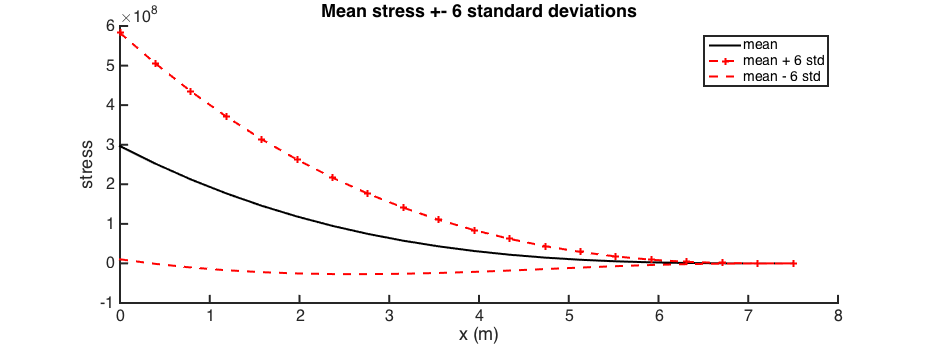
\includegraphics[width=0.95\textwidth]{nominal_stress}
\caption{Computed nominal stresses}
\label{fig:nominal_stress}
\end{minipage}%
\begin{minipage}[b]{0.5\textwidth}
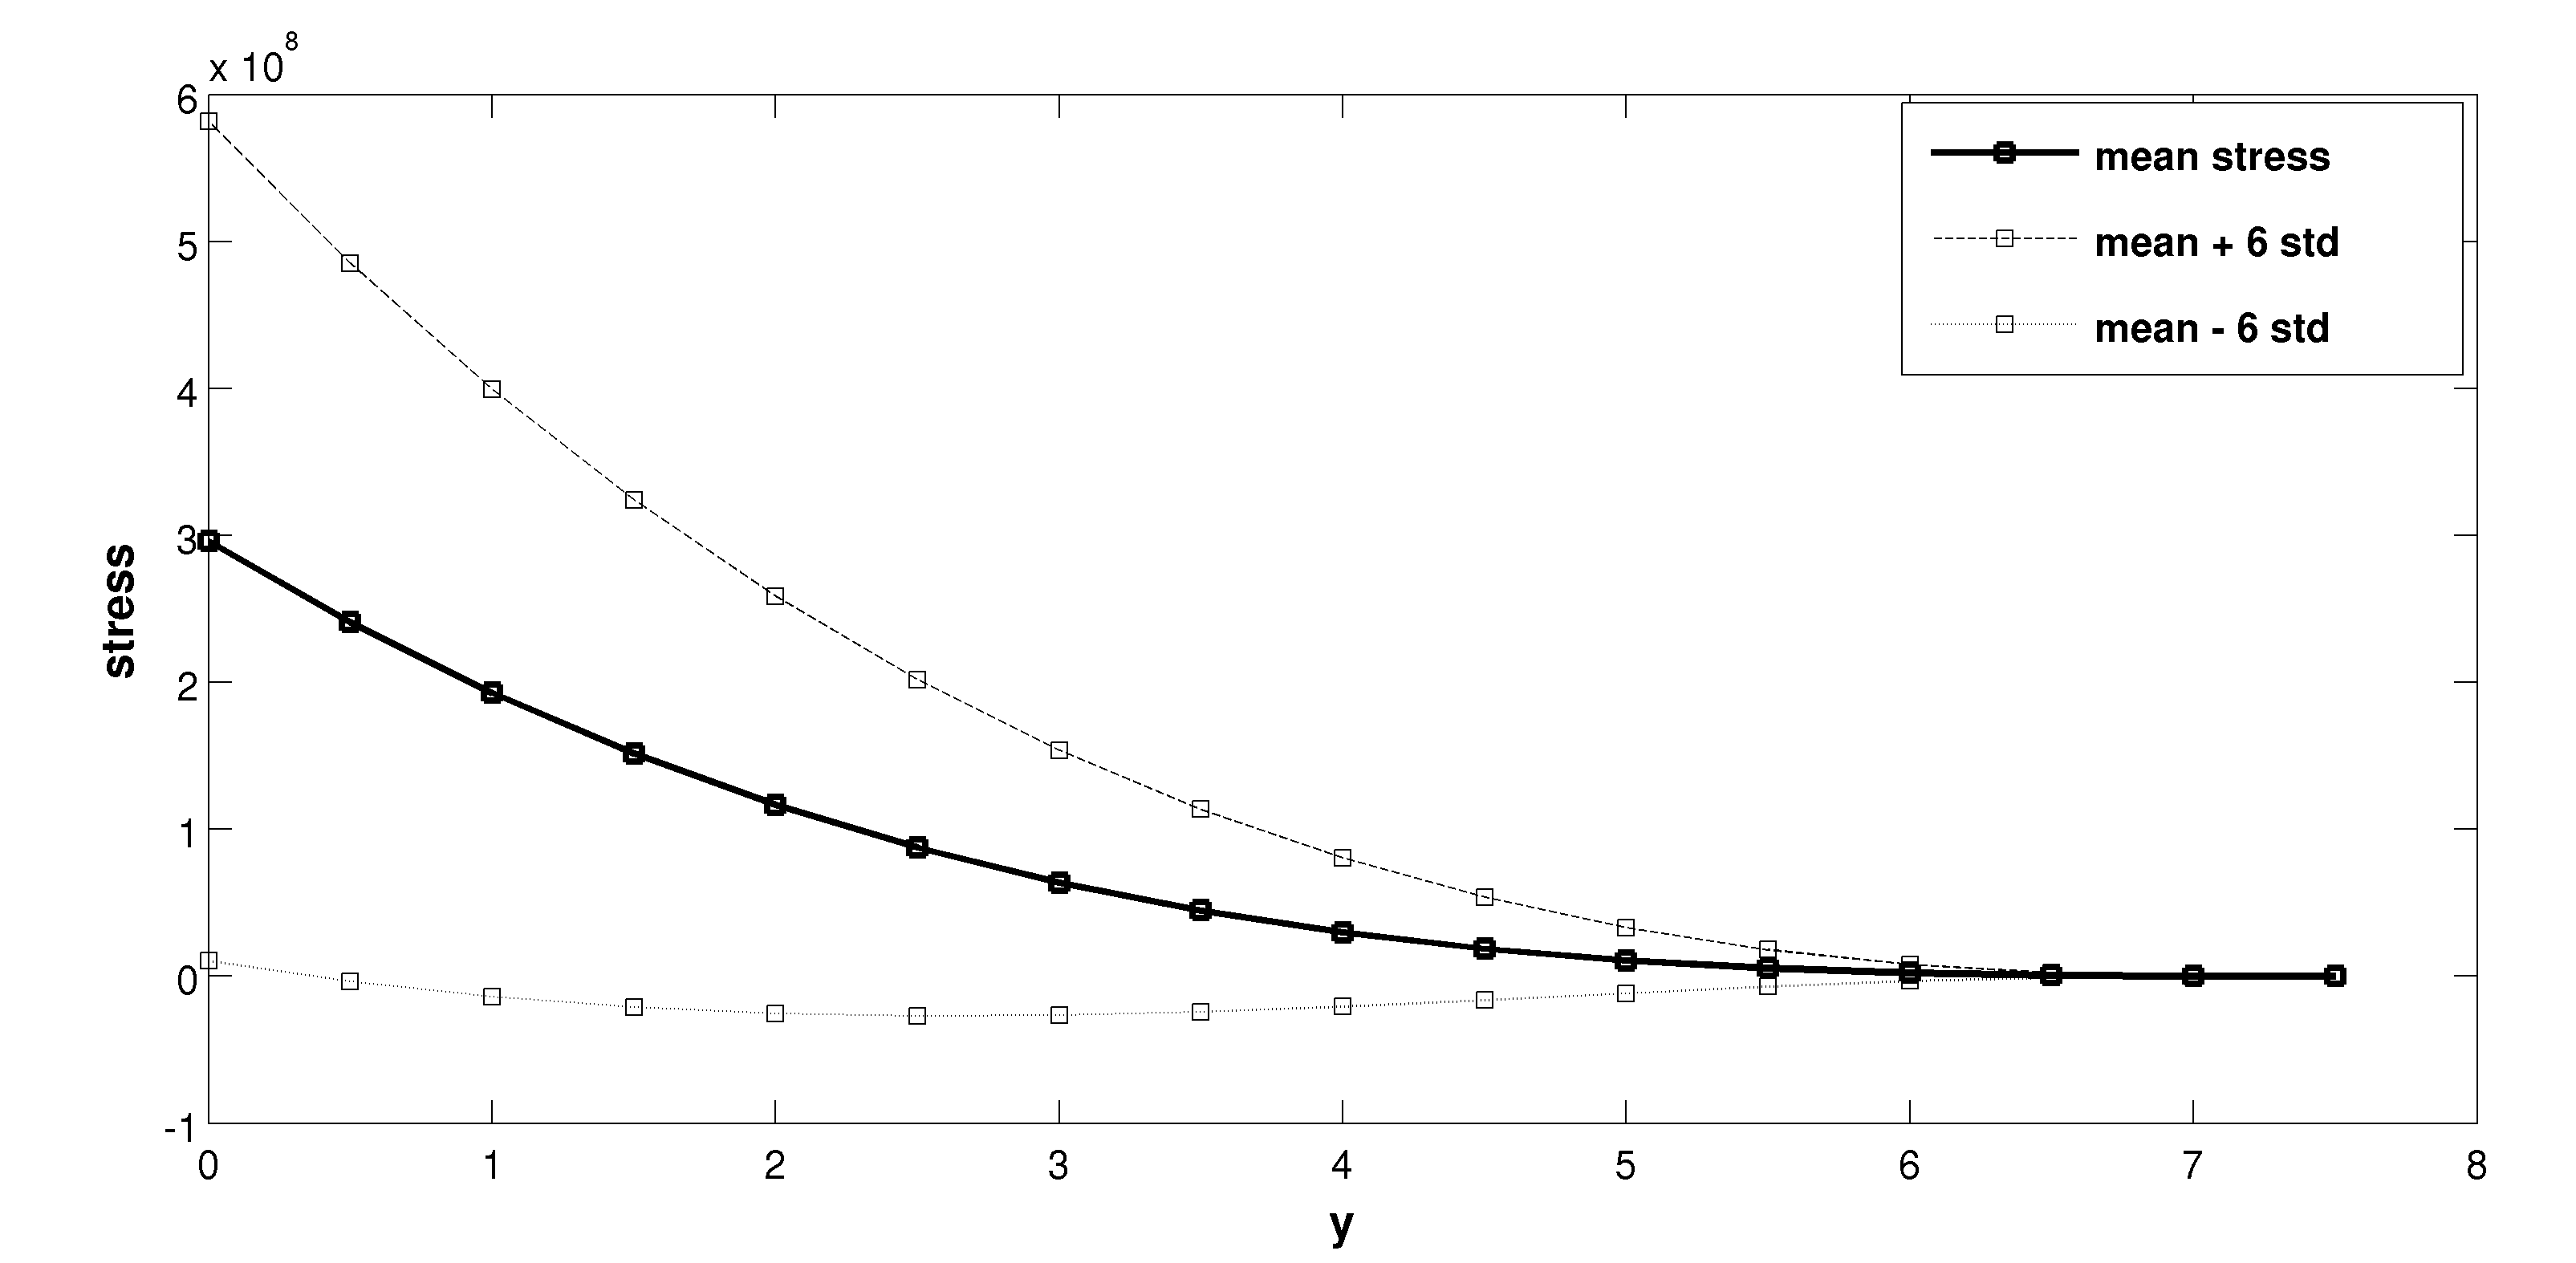
\includegraphics[width=0.8\textwidth]{nominal_stress_hicken}
\caption{Known nominal stresses}
\label{fig:nominal_stress_hicken}
\end{minipage}
\end{figure}

The convergence history for the optimization routine
is shown below. The value of the spar mass computed for the
nominal geometry is $29.32$ kg, which agrees with a known value
presented to us independently. The optimal spar's mass of $8.57$ kg
is just over 70 percent lighter than the nominal spar's mass,
achieving our desired optimization goal.
%
\begin{figure}[hbt!]
\scriptsize
\begin{verbatim}
 Iter F-count            f(x) Feasibility  Steplength        step  optimality
    0       1    2.932048e+01   0.000e+00                           1.984e+02
    1       3    1.032301e+01   1.611e+00   7.000e-01   8.323e-02   6.197e+02
    2       4    7.908339e+00   1.496e+00   1.000e+00   3.763e-02   3.860e+02
    3       5    8.404552e+00   4.704e-01   1.000e+00   1.359e-02   6.832e+01
    4       6    8.559594e+00   8.094e-02   1.000e+00   5.516e-03   9.968e+00
    5       7    8.574724e+00   3.297e-03   1.000e+00   8.917e-04   2.276e+00
    6       8    8.574903e+00   5.853e-06   1.000e+00   2.931e-05   9.966e-02
    7       9    8.574903e+00   1.878e-11   1.000e+00   4.824e-08   4.693e-05
\end{verbatim}
\label{fig:convergence}
\end{figure}

Figure \ref{fig:nominal_geom} shows the nominal spar geometry
and Figure \ref{fig:optimal_geom} shows the computed optimal spar
geometry. Notice that the optimal spar is quite thick towards
its junction with the fuselage of the plane and tapers down
gradually along the length of the spar until the minimum
thickness constraint is reached.
%
\begin{figure}[hbt!]
\centering
\begin{minipage}[b]{0.4\textwidth}
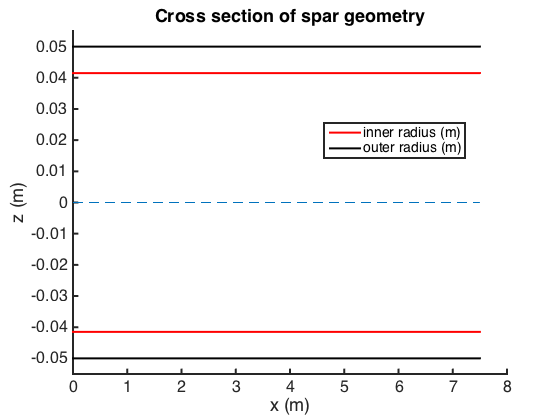
\includegraphics[width=0.9\textwidth]{nominal_geom}
\caption{Nominal spar geometry}
\label{fig:nominal_geom}
\end{minipage}
\begin{minipage}[b]{0.4\textwidth}
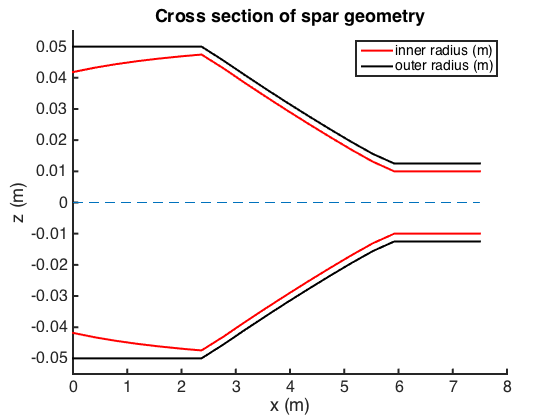
\includegraphics[width=0.9\textwidth]{optimal_geom}
\caption{Optimal spar geometry}
\label{fig:optimal_geom}
\end{minipage}
\end{figure}

Figure \ref{fig:optimal_stress} shows the mean stress computed
for the optimal spar, as well as the mean stress plus or minus
six standard deviations. It is immediately clear that the
nonlinear stress constraint has been satisfied, where the
mean stress plus six standard deviations is at all points
along the spar less than the yield stress $Y$. This leads
to further confidence that
we have solved the optimization problem
correctly, and is congruent with engineering intuition.
%
\begin{figure}[hbt!]
\centering
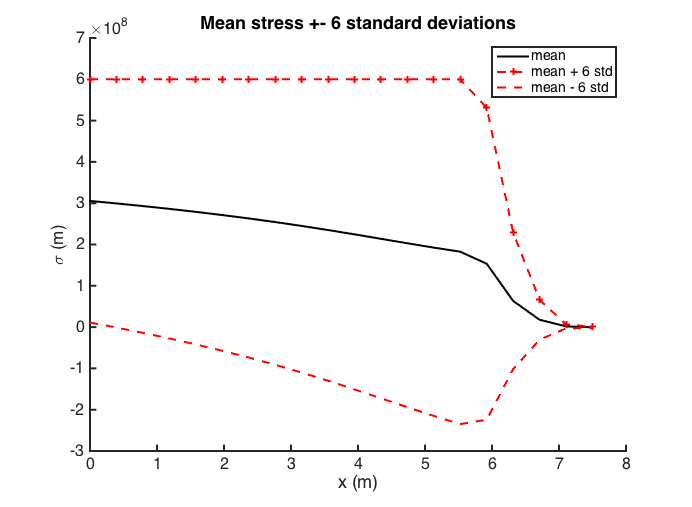
\includegraphics[width=0.5\textwidth]{optimal_stress}
\caption{Optimal spar stress distribution}
\label{fig:optimal_stress}
\end{figure}

\section{Conclusions}

We have investigated the optimal design of a wing
spar under uncertain loading conditions. Using
gradient-based optimization with 
stochastic collocation techniques, we have minimized the mass of
the wing spar so that normal stresses along spar are
considered safe during a variety of loading conditions.
The optimal geometry's mass was found to be over 70
percent less than the mass of a nominal geometry,
achieving the desired goals of this optimization
project.

\newpage

\section{Appendix : code listings}

\lstinputlisting[style=matlab-style,caption=CalcWeight.m]{CalcWeight.m}
\newpage
\lstinputlisting[style=matlab-style,caption=CalcQPs.m]{CalcQPs.m}
\newpage
\lstinputlisting[style=matlab-style,caption=StressConstraints.m]{StressConstraints.m}
\newpage
\lstinputlisting[style=matlab-style,caption=Plotter.m]{Plotter.m}
\newpage
\lstinputlisting[style=matlab-style,caption=Driver.m]{Driver.m}

\end{document}
